\documentclass[10pt,twocolumn]{article}

%%% packages %%%
\usepackage{color}
\usepackage{graphicx}
\usepackage{listings}
\usepackage{float}
\usepackage{url}
\usepackage{times}
\usepackage{xspace}
\usepackage{microtype}
\begin{document}

\title{SSA Construction and Optimization\ \\
  \small CSE 501 Spring 2013 Compilers Assignment 2}
\author{Andre Baixo, Jacob Nelson}
\maketitle

This writeup describes our optimizer implementation for Assignment 2.

\section{Implementation}

Our optimizer implements 

\paragraph{Conversion from SSA} We use the naive approach, 
replacing phi functions with writes to temporary variables. We follow
this with a pass that promotes most SSA variables to registers 

\paragraph{Code generation} We use the naive approach to c




Besides the generated code, our optimizer writes two forms of
debugging output. First, it dumps the all the requested information
about blocks, instructions, and dominators to a file. Second, it
writes the CFGs in GraphViz format. This may be converted to a
graphical representation using the \texttt{dot} program.

\section{Running}

The optimizer may be run by executing the \texttt{assignment2/run.rb}
script while inside the \texttt{assignment2} directory. We have
included precompiled intermediate languages files for all examples in
the distribution. Running the script will create separate output files
in the \texttt{examples} directory for each method of each example;
optimized intermediate language output has the extension
\texttt{.ilo}, dump information has the extension \texttt{.txt}, and
CFG output has the extension \texttt{.dot}. For example, the results
for the GCD method in \texttt{gdc.dart} can be found in
\texttt{examples/gcd.dart.il-main-info.txt}. The GraphViz files can be
turned into PDF with a command like \texttt{dot -Tpdf file.dot >
  file.pdf}.

Our optimizer is implemented in Ruby, so no separate build step is
required. Ruby version 1.9 is required.

\section{Examples}

\begin{figure}
\begin{center}
  \includegraphics[width=0.95\columnwidth]{figs/hammock.pdf}
\begin{minipage}{0.95\columnwidth}
  \caption{\label{fig:hammock} CFG from hammock example. Red edges show dominator relationships.}
\end{minipage}
\end{center}
\end{figure}

\begin{figure}
\begin{center}
  \includegraphics[width=0.95\columnwidth]{figs/weave.pdf}
\begin{minipage}{0.95\columnwidth}
  \caption{\label{fig:weave} CFG from weave example. Red edges show dominator relationships.}
\end{minipage}
\end{center}
\end{figure}

\begin{figure}
\begin{center}
  \includegraphics[height=6in]{figs/nested-if-10-1.pdf}
  \caption{CFG from 10-if singly-nested example. Red edges show dominator relationships.}
  \label{fig:nest-10-1}
\end{center}
\end{figure}

\begin{figure}
\begin{center}
  \includegraphics[height=6in]{figs/nested-if-10-5.pdf}
  \caption{CFG from 10-if 5-nested example. Red edges show dominator relationships.}
  \label{fig:nest-10-5} 
\end{center}
\end{figure}

\begin{figure}
\begin{center}
  \includegraphics[height=6in]{figs/nested-if-10-10.pdf}
  \caption{CFG from 10-if 10-nested example. Red edges show dominator relationships.}
  \label{fig:nest-10-10} 
\end{center}
\end{figure}

We implemented three additional examples to better understand our
implementation. The first is \texttt{examples/hammock.il}, a simple
dual hammock shown in Figure~\ref{fig:hammock}. The second is
\texttt{examples/weave.il}, a more complicated set of woven branches
shown in Figure~\ref{fig:weave}. Both of these examples provide a simple
verification of our dominator construction.

The third example is a script that generates nested {\it if}
constructs of different sizes. The Ruby file
\texttt{examples/nested-if.rb} takes two parameters: a total
if-construct count, and a nesting depth. The nesting depth controls
how many levels of nested if constructs are generated.
Figure~\ref{fig:nest-10-1} shows a CFG from a 10-node, singly-nested
example; figure~\ref{fig:nest-10-5} shows a 10-node, 5-nested example,
and figure~\ref{fig:nest-10-10} shows a 10-node, 10-nested
example. This lets us generate different families of programs with
different numbers of nodes and edges, as well as different patterns of
CFG connectivity. In Section~\ref{eval}, we use this script to explore
how the structure of the CFG affects runtime.

\section{Results}
\label{eval}


We explored the performance of our implementation in three ways. For
all our experiments, we ran on an Ivy Bridge-based MacBook Air with
8GB of RAM.

First, we processed all the example programs provided. The
longest-running method was the main method from \texttt{mmm.dart},
which ran for about 200 microseconds. The examples can be run by
executing the \texttt{assignment1/run.sh} script. This 

Since this time is too short to make meaningful comparisons, we then
used our nested-if generator to create a set of larger programs with
different CFG shapes. Unfortunately we were hampered by our
implementation choices: by depending on the Ruby VM stack for
computing a topological order, we were limited to CFGs whose depth was
on the order of 2000 nodes. This could be easily avoided by modifying
the code to use an external stack for the traversal, but since we
expect that real programs are rarely nested this deep, we chose not to
do this.


\begin{figure}
\begin{center}
  \includegraphics[width=0.95\columnwidth]{figs/g1.pdf}
\begin{minipage}{0.95\columnwidth}
  \caption{\label{fig:nodes} Relationship between CFG node count and runtime in nested if example with nesting depth of 1.}
\end{minipage}
\end{center}
\end{figure}

The first experiment we ran with the nested if generator was intended
to show the cost of scaling the size of the CFG. In this experiment,
we varied the number of nodes and edges together while keeping the
nesting depth fixed at 1. Figure~\ref{fig:nodes} shows the result. We
find that runtime varies linearly with the number of nodes and edges.


\begin{figure}
\begin{center}
  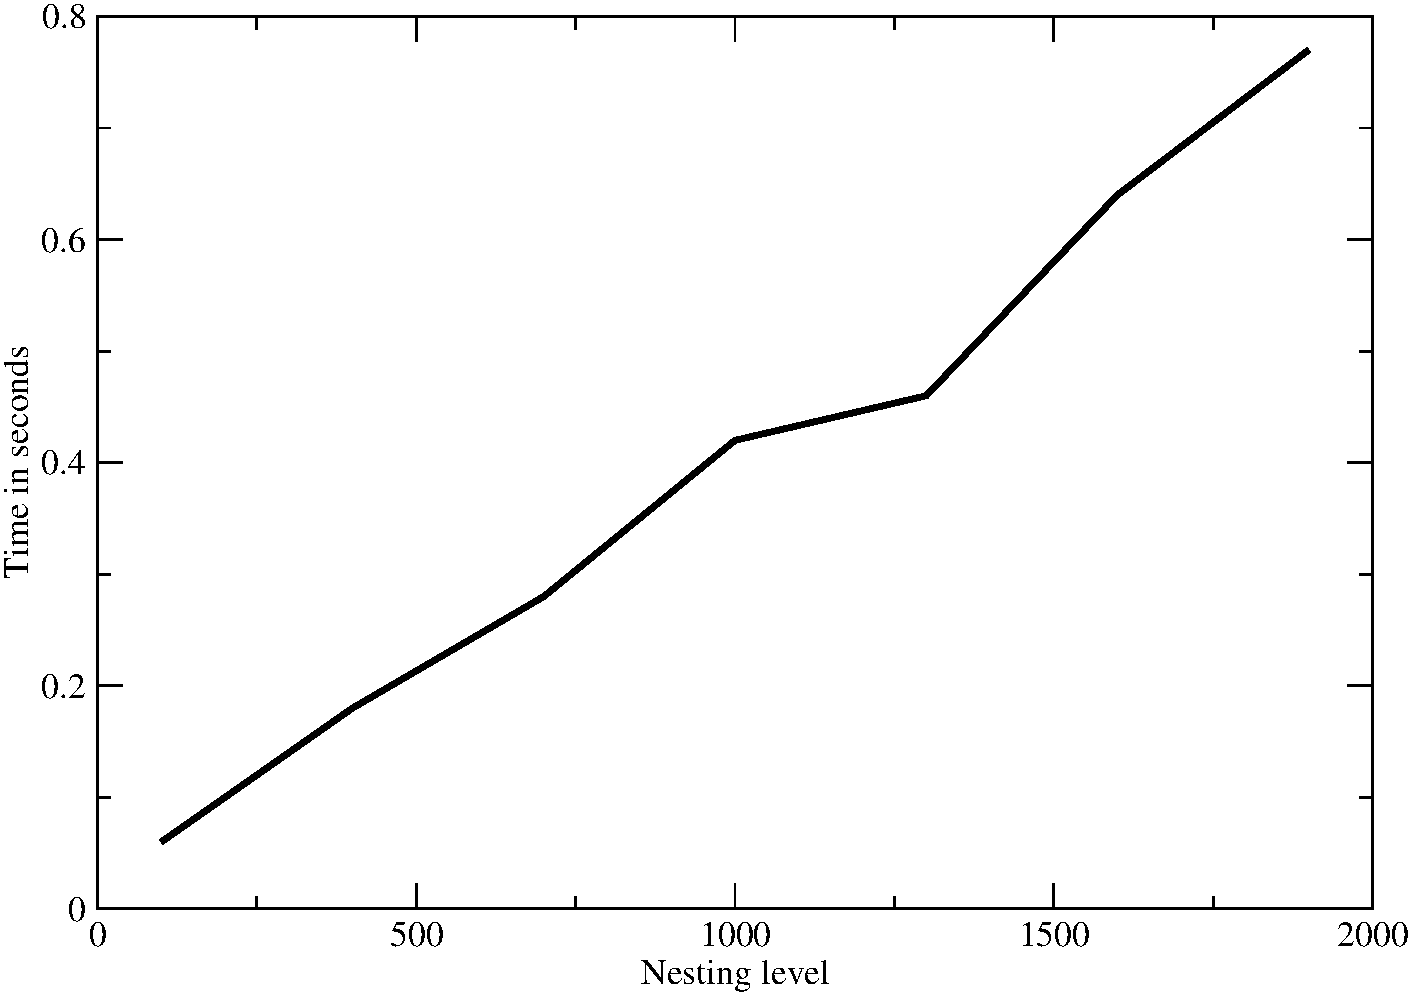
\includegraphics[width=0.95\columnwidth]{figs/nesting.pdf}
\begin{minipage}{0.95\columnwidth}
  \caption{\label{fig:nesting} Relationship between nesting depth and runtime in nested if example.}
\end{minipage}
\end{center}
\end{figure}

The second experiment we ran with the nested if generator was intended
to show that varying the structure of the graph given a constant node
and edge count has a significant impact runtime. In this experiment,
we held the node count fixed at 4000 and varied the depth of the
nested if blocks. Figure~\ref{fig:nesting} shows the result. We find
that runtime varies linearly with the depth of nesting. This shows
that for the dominance algorithm we implemented, it is insufficient to
describe its performance only in terms of nodes and edges---the
structure of the CFG has a significant effect on its performance.

\section{Conclusion}

We implemented a dominance algorithm for the Start intermediate
language. We found that the algorithm performs well for our example
programs, and that the structure of the CFG has a significant effect
on the performance of dominance detection.

\bibliographystyle{abbrv}
\bibliography{writeup}

\end{document}

